%%%
 % File:     buffer_overflow.tex
 % Author:   Hackademics Forum <hackademicsforum6@gmail.com>
 % Project:  MindMap des vulnérabilités
 % Released: 03/08/2016
%%%

%!TeX root = main.tex
%!TeX encoding = UTF-8
%!TeX program = pdflatex
%!TeX spellcheck = fr_FR

%%%
 % Vulnérabilités Buffer Overflow
%%%
\newpage
\section{Dépassement de tampon (Buffer Overflow)}\label{vulnerabilites:applicatives:buffer-overflow}

Un Buffer Overflow ou dépassement de tampon se produit lorsque un programme ou un processus tente de stocker plus de données dans une mémoire tampon (stockage temporaire) que prévue par celle-ci. Ces mémoires tampon sont prévues pour accueillir une quantité limitée de données. Les informations supplémentaires qui doivent bien être stockées quelque part se retrouvent dans des tampons adjacents. Les données déjà stockées dans ces tampons sont à ce moment écrasées et endommagée. Bien que cela puisse également se produire accidentellement en raison d'une erreur de programmation, les dépassements de tampon sont de plus en plus utilisés pour volontairement corrompre les données. Dans des attaques ciblées par débordement de tampon,   ces informations complémentaires peuvent contenir du code malveillant qui déclenchera des actions spécifiques sur le système attaqué. Par exemple le code peut contenir des instructions qui peuvent endommager des fichiers sur le pc, simplement modifier des données ou mener au vol de certains renseignements intéressants.


\subsection{Stack Overflow}\label{vulnerabilites:applicatives:buffer-overflow:stack}

Chez les processeurs X86, le STACK commence a l’extrémité supérieure de la mémoire (ex:0xffffffff) et pousse vers le bas (vers 0x00000000). Le mot STACK viens de l'anglais et veut dire PILE. Il se nomme ainsi car il se comporte en LIFO (Last In First Out): si quelque chose est ajouté (PUSH,écriture), la PILE est augmentée, au contraire si quelque chose est lu (POP), la PILE est abaissée: l'élément est lu et supprimé. Il existe une troisième méthode nommée TOP ou PEEK, ou l'élément est simplement lu mais pas supprimé. Le pointeur de PILE (ESP) est toujours à la dernière adresse de la PILE.

\begin{center}
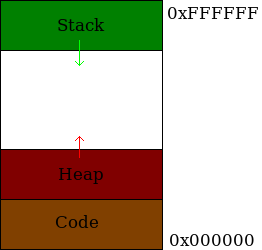
\includegraphics[scale=0.5]{Application/assets/stack.png}
\end{center}

\begin{flushleft}
Le programme ci-dessous simule le scénario où un programme attend un mot de passe de l'utilisateur. Si le mot de passe est correct,des privilèges root sont accordés à l'utilisateur.
\end{flushleft}

\begin{center}
<<<<<<< HEAD
\includegraphics[scale=0.5]{/home/nait/Bureau/mindmap/MindMap/latex/Application/assets/codebo.png}
=======
\vspace{0.5cm}
\includegraphics[scale=0.3]{Application/assets/codebo.png}
\vspace{0.5cm}
>>>>>>> 2142cffc0880e114c48bcb7adec010a6677a09ac
\end{center}

\begin{flushleft}
\textbf{Démarrons le programme avec le mot de passe : ‘hackademics'}
\end{flushleft}

\begin{center}
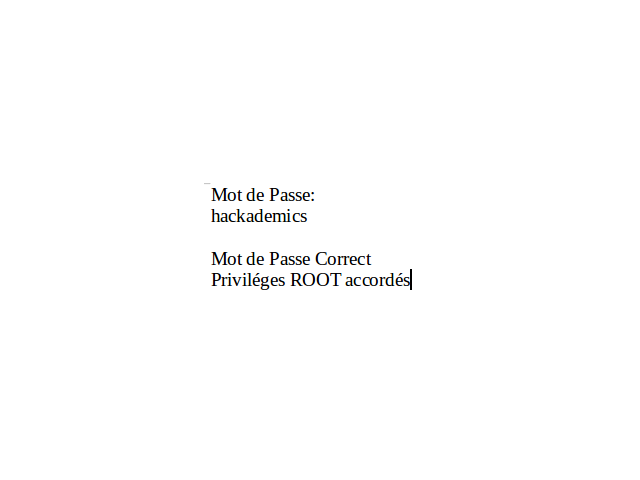
\includegraphics[scale=0.5]{Application/assets/bmdp.png}
\end{center}

\begin{flushleft}
Le programme fonctionne comme prévu. Le mot de passe correspond et les privilèges root sont donnés.Mais savez-vous qu'il y a un risque de Buffer Overflow dans ce programme. La fonction gets () ne vérifie pas les limites du tableau et peut ainsi permettre d'écrire une chaîne de longueur supérieure à la taille de la mémoire tampon. Maintenant, vous pouvez vous imaginer ce que peut faire une personne mal intentionnée avec ce genre de vulnérabilité.
\end{flushleft}


\begin{flushleft}
\textbf{Voici un exemple:}
\end{flushleft}

\begin{center}
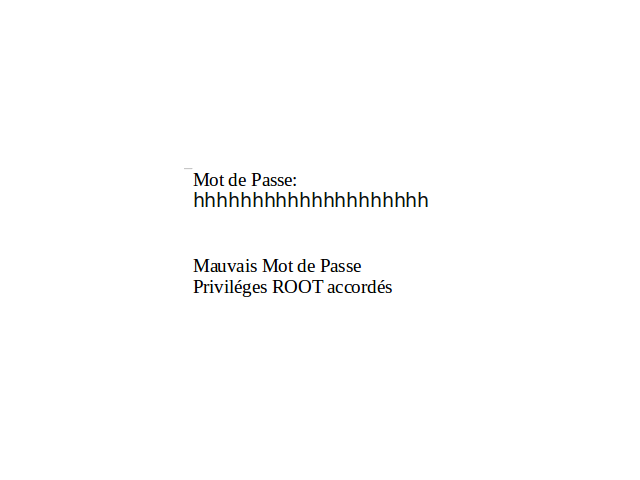
\includegraphics[scale=0.5]{Application/assets/mmdp.png}
\end{center}

\begin{flushleft}
Dans l'exemple ci-dessus, même après la saisie d'un mot de passe incorrect, le programme a fonctionné comme si le bon mot de passe avait été entré.
Ce que l'utilisateur a fait, est qu'il a entré une chaine de caractères plus grande que prévue par la mémoire tampon. La valeur de "Mot de Passe" a donc été écrasée et a été passée a non nul. Ainsi en dépit d'un mauvais mot de passe, le privilèges ROOT ont été accordés.
\end{flushleft}

\begin{flushleft}
\textbf{Comment déterminer si vous êtes vulnérable.}
\end{flushleft}

\begin{flushleft}
Si votre programme:
est écrit dans une langue (ou dépend d'un programme qui est écrit dans une langue) qui permet de copier des données d'un buffer sur le stack vers un autre sans en vérifier au préalable la taille et qui n'utilise pas de valeurs canaries ou de stack non-executable pour éviter un Buffer Overflow. Il est probable que l'application soit vulnérable à un dépassement de tampon.
\end{flushleft}

\begin{flushleft}
Pour éviter un dépassement de tampon, les conseils généraux pour les développeurs sont de suivre de bonnes pratiques de programmation comme par exemple: 
\end{flushleft}
\begin{flushleft}
Assurez-vous que la vérification de la mémoire se fait correctement dans le programme à l'aide des utilitaires comme valgrind memcheck.
Utilisez fgets () au lieu de gets ().
Utilisez strncmp () au lieu de strcmp (), strncpy () au lieu de strcpy () et ainsi de suite. déployer sur des systèmes capables d'utiliser des piles non exécutables, tels que:Des puces AMD et Intel x86-64  avec les systèmes d'exploitation 64 bits associés.
Utilisez des langages de programmation de plus haut niveau qui sont fortement typés et qui interdisent l'accès direct à la mémoire.
Valider l'entrée pour empêcher  des données inattendues d'être traitées, comme étant trop longue, ou de type de données incorrect, contenant des caractères "junk", etc.
utiliser le principe du moindre privilège
utiliser des compilateurs qui protègent contre les Buffer Overflow 
<<<<<<< HEAD
\end{flushleft}
=======

>>>>>>> 2142cffc0880e114c48bcb7adec010a6677a09ac

\subsection{Heap Overflow}\label{vulnerabilites:applicatives:buffer-overflow:heap}


